\documentclass{cmspaper}
\usepackage{lineno}
\usepackage{amsfonts,amsmath,amssymb}
\usepackage[dvips]{graphicx}
\usepackage{bm}
\begin{document}
\begin{linenumbers}

\begin{titlepage}

\cmspas{EXO-09-0XX}
%  \internalnote{2005/000}
%  \conferencereport{2005/000}

%\begin{center}
%{\bf \huge  CMS Physics Analysis Summary }
%\end{center}

\date{\today}

\title{Search for Pair Production of First Generation Scalar Leptoquarks at the CMS Experiment}


  \begin{Authlist}
%   Sarah Eno, Paolo Rumerio, Francesco Santanastasio, Elizabeth Twedt
    The CMS Collaboration, CERN
    %\Instfoot{cern}{University of Maryland, College Park, MD, USA}
  \end{Authlist}


  \begin{abstract}
    The discovery potential for pair production of first generation scalar leptoquarks that 
    decay to an electron and quark is investigated 
    at the CMS experiment using Monte Carlo samples produced with a full simulation of detector response.  
    The analysis strategy assumes an integrated luminosity of 100 pb$^{-1}$ and $pp$ collisions 
    at $\sqrt{s}=10$ TeV.
    Reconstruction and identification of high energy electrons and jets, 
    and optimized selection of events are discussed.
    The electron-jet invariant mass distribution is reconstructed
    and used to identify the possible presence of a leptoquark signal.
    Data-driven techiques are discussed to determine the main standard model backgrounds through use of 
    control samples. The CMS discovery and exclusion potentials using a counting experiment approach 
    are quantified for different leptoquark mass hyphotheses.

%The leptoquarks are assumed to decay exclusively to electrons and quarks.  Detailed explanations of the discovery techniques and data driven methods to extract the signal from background events are given.  
%Both exclusion limits and discovery potential are discussed for masses of the leptoquark ranging from around the current limit of 251 GeV to 1 TeV.
  \end{abstract} 

\end{titlepage}

%=================================================================
\setcounter{page}{2}%JPP

\section{Introduction}
 
This note describes the analysis techniques that will be used to search for evidence of first generation scalar leptoquarks 
at the CMS experiment. The methods described are evaluated using Monte Carlo (MC) simulations assuming a start-up LHC scenario
with about 100 pb$^{-1}$ of integrated luminosity and 5 TeV proton beams.

Leptoquarks (LQ) are new exotic particles conjectured to have both baryon and lepton number and primary decays into leptons and quarks.    
Several models of physics beyond the standard model (SM) predict the existence of leptoquarks, including General Unified Theories, 
technicolor and composite models \cite{theories}.  

The parameters of the model are i) $M_{LQ}$, the LQ mass, ii) $\beta$, the branching fraction for the decay 
$\mbox{LQ} \rightarrow l + q$, where $l$ is a charged lepton and $q$ is a quark, and
iii) $\lambda_{\mbox{LQ}lq}$, the coupling between LQ, lepton and quark ($\mbox{LQ}-l-q$ vertex). 
The complementary decay of a branching ratio 1-$\beta$ describes the decay $\mbox{LQ} \rightarrow \nu + q$, 
where $\nu$ is a weak-isospin partner of the lepton.
Results from HERA on upper limits for LQ production restrict  
$\lambda_{\mbox{LQ}lq}$ to relatively weak coupling\cite{hera}. For example, fixing the parameter 
$\lambda_{\mbox{LQ}lq} = \lambda_{EM} \approx 0.3$, leads to 
a theoretical relative width for the LQ of ($\Gamma_{LQ}/M_{LQ}$) around 0.2\%. 
Consequently, $\Gamma_{LQ}/M_{LQ}$ will not be able to be measured at the LHC, since 
the width of any peak on the mass distribution of the LQ will be dominated by detector resolution.  

Experiments at the Tevatron have placed the most stringent lower limit on the mass of first-generation scalar 
leptoquarks of approximately 290 GeV (assuming $\beta=1$ for the electron channel) \cite{d02008},\cite{cdf2005}.
At the LHC, the pair production of leptoquarks will take place mainly through gluon-gluon fusion and 
quark-antiquark annihilation, yielding $LQ + \overline{LQ}$. 
The cross sections for the two sub-processes are almost independent on the value of 
$\lambda_{\mbox{LQ}lq}$, since there is no $\mbox{LQ}-l-q$ vertex in the Feynman diagram for LQ pair production 
at leading order. At lower rate, the production of single leptoquark in association with a lepton is also possible via quark-gluon 
fusion, yielding $LQ+ l$ or $LQ+ \nu$ (and relative final states with antiparticles). The cross section of single leptoquark production
becomes comparable to the one of pair production only for $M_{LQ}\approx 1$ TeV \cite{LQSingleAndPairProd}, 
which is well above the experimental reach of this start-up analysis (focused on the first 100 pb$^{-1}$ of data at $\sqrt{s}=10$ TeV).  
This note examines the signal for pair production of first-generation scalar leptoquarks that decay into electrons and 
(light) quarks with a branching ratio $\beta=1$. 
For this scenario, the experimental signature of a LQ event is quite striking with two 
high transverse momentum ($p_T$) electrons and two high $p_T$ jets (eejj channel), 
whose combination yields a peak in the electron-jet invariant mass 
spectrum that corresponds to the LQ mass. No true missing transverse momentum is expected in LQ events.


\section{Monte Carlo Samples} \label{sec:MCSamples}
MC signal samples are generated with leptoquark masses ranging from 250 to 600 GeV and $\beta=1$. 
At the LHC, the three main processes that lead to leptoquark pair production are gluon-gluon fusion, 
quark-antiquark annihilation, and the higher order process of quark-gluon fusion. In the mass range to be investigated gluon-gluon fusion dominates. 

The ``Full Simulation'' (FullSim) signal samples are produced using 
the official CMS software for generation (using PYTHIA version 6.227), 
simulation (based on GEANT4), digitization and reconstruction. 
%The above lines are taken from the previous version of the PAS, instead of from the note.
These samples were included in the official ``Summer 08'' production by the CMS Generators group.

``Fast simulation'' (FastSim) signal samples are produced with a slightly later version of the CMS software.
The FastSim uses a parameterization of the detector response instead of using the full GEANT-based simulation.
The FastSim samples were created during the ``Winter 09'' production campaign by the CMS Generators group.

The SM background is taken from the Summer08 official production samples,
which consists of more than 200M events of various SM processes roughly representing 
the first 100 pb$^{-1}$ of LHC data. The Summer08 samples used for this analysis are listed below:
\begin{itemize}
%
\item $t\bar{t}$+jet events (for N$<$5), generated using MADGRAPH~\cite{MADGRAPH}, inclusive production (all decays); 
%with a LO-NLO K correction factor of 1.85 applied to the LQ cross section;\footnote{The K factor of 1.85 applied 
%to ttbar events is a default in the software provided by CMS for these data samples.  It is from a MCFM NLO vs LO study.}
%
\item $Z/\gamma*$ + N jet events (for N$<$6), generated using MADGRAPH, $Z$ decaying into charged leptons;  
%
\item $W$ + N jet events (for N$<$6), generated using MADGRAPH, $W$ decaying into leptons; 
% $0< P_{T}^{W} < 300 $ GeV (FIXME)
%
%\item QCD multi-jet events, generated with PYTHIA, inclusive production in $P_{T}^{jet}$ bins from 0 to $\infty$;  
\item QCD multi-jet events, generated with MADGRAPH, inclusive production in 
$H_{T}^{jet}$~\footnote{$H_{T}^{jet}=\sum_{jets} p_T^{jet}$} bins from 100~GeV to 1~TeV;  
%
%\item $\gamma$+jet events, generated with PYTHIA, $ 0 < P_{T}^{jet} < 7000 $ GeV;  
%
%\item $WW$, $WZ$, $ZZ$ events, generated with PYTHIA, inclusive production (all decays).
\item $VV$ + jet events (where $VV$ can be $WW$, $WZ$ or $ZZ$), generated with MADGRAPH, $W$ and $Z$ 
decaying into leptons.
\end{itemize} 

Table~1
%\ref{tab:NumEvents} 
lists the signal and background MC samples used in this analysis with their number of events and cross sections.
%shows the number of events and the cross sections at leading order (LO) for samples generated at different LQ mass.

\begin{table}[htb]
  \label{tab:NumEvents}
  \begin{center}
    \begin{tabular}{|l|cccccc|} \hline\hline
%      & \multicolumn{4}{c|}{Leptoquark Mass (GeV)} \\ 
      MC Sample                   & Full/Fast & N. Events & Equivalent             & $\sigma_{NLO}$ (pb) & $\sigma_{LO}$ (pb) & K-factor \\
                                  & Simulation& Analyzed  & Luminosity (pb)        &                     &                    &    \\ 
\hline\hline
      $M_{LQ}=250~$GeV            & Full      & 52k       &    5.15$\times 10^3$   & 10.1                & 6.53               & 1.547\\
      $M_{LQ}=400~$GeV            & Full      & 63k       &      84$\times 10^3$   &  0.75		 & 0.462	      & 1.628\\ 
\hline
      $M_{LQ}=250~$GeV            & Fast      & 125k      &    12.4$\times 10^3$   & 10.1		 & 6.53		      & 1.547\\
      $M_{LQ}=300~$GeV            & Fast      & 127k      &    33.4$\times 10^3$   &  3.8	         & 2.42		      & 1.57\\
      $M_{LQ}=400~$GeV            & Fast      & 150k      &     200$\times 10^3$   &  0.75	         & 0.462	      & 1.628\\
      $M_{LQ}=500~$GeV            & Fast      & 125k      &     635$\times 10^3$   &  0.197  	         & 0.118	      & 1.669\\
      $M_{LQ}=600~$GeV            & Fast      & 131k      &    2.12$\times 10^6$   &  0.0617             & 0.0617             & 1.723\\
%      $M_{LQ}=650~$GeV            & Fast      & 133k      &    3.67$\times 10^6$  &  0.0362 	         & 0.0208	      & 1.740\\
%      $M_{LQ}=700~$GeV            & Fast      & 146k      &    6.70$\times 10^6$  &  0.0218 	         & 0.0124	      & 1.758\\
%      $M_{LQ}=800~$GeV            & Fast      & 146k      &    17.2$\times 10^6$  &  0.0085 	         & 0.00466	      & 1.815\\
%      $M_{LQ}=900~$GeV            & Fast      & 146k      &    41.6$\times 10^6$  &  0.00351	         & 0.00188	      & 1.867\\
%      $M_{LQ}=1000~$GeV           & Fast      & 146k      &    95.4$\times 10^6$  &  0.00153            & 0.000794           & 1.927\\ 
%      $M_{LQ}=1200~$GeV           & Fast      & $>$100k   &                       &  0.000329           & 0.000158           & 2.082\\
%      $M_{LQ}=1500~$GeV           & Fast      & $>$100k   &                       &  0.0000393          & 0.0000165          & 2.382\\ \hline
\hline
      $t\bar{t}$ + N jets         & Full      & 0.905M    &    2.19$\times 10^3$   & 414                 &  317                  & 1.31 \\
      $Z/\gamma$ + N jets         & Full      & 1.159M    &    275	           & 4218                &  3700                 & 1.14 (@14 TeV)\\
      $Z/\gamma$ + N jets         & Fast      & 8.46M     &    2$\times 10^3$      & 4218                &  3700                 & 1.14 (@14 TeV)\\
      $W$ + N jets                & Full      & 6.107M    &     134	           & 45600               &  40000                & 1.14 (@14 TeV)\\
      $VV$ + N jets               & Full      & 101.8k    &    8.63$\times 10^3$   &                     &  11.8                 & \\ \hline
      QCD ($H_T\in[100,250]$~GeV) & Full      & 13.721M   &    0.915	           &                     &  $15.0 \times 10^6$   & \\
      QCD ($H_T\in[250,500]$~GeV) & Full      & 3.698M    &    9.25	           &                     &  $400 \times 10^3$    & \\
      QCD ($H_T\in[500,1000]$~GeV)& Full      & 3.807M    &     272	           &                     &  $14 \times 10^3$     & \\
      QCD ($H_T>1000$~GeV)        & Full      & 0.654M    &    1.77$\times 10^3$   &                     &  $370$                & \\
\hline\hline
    \end{tabular}
    \caption{\small \sl Signal and background MC samples used in this analysis. For each sample, it is indicated 
      if it is generated with the full or fast simulation, the generated number events, 
      and the cross sections at NLO and LO for $\sqrt{s}=10$ TeV. 
      The k-factor is also reported for convenience. Leptoquark cross sections at NLO and LO
      are given based on the calculation discussed at~\cite{Kramer} (thanks to Micheal Kramer 
      for providing the updated numbers for $\sqrt{s}=10$ TeV).}
  \end{center}
\end{table}

\section{Trigger Studies} \label{sec:trig}

The presence of two high energy electrons in the final state is exploited for the online selection 
of candidate leptoquark-antileptoquark events.

Two trigger menus, named ``8E29'' and ``1E31'', have been studied and designed as candidates for 
the two possible luminosity scenario of the CMS start-up.
% More, if needed, at https://twiki.cern.ch/twiki/bin/view/CMS/TSG_18_II_09
In case that the ``8E29'' menu is used, the chosen trigger would be the ``HLT\_Photon15\_L1R''.
The corresponding Level-1 trigger seed is ``L1\_SingleEG8'', which requires an electromagnetic object with 
$E_T>8~$GeV. At the HLT level, the threshold applied is $E_T>15~$GeV and no isolation or track-matching
are required.
If the ``1E31'' menu is used, the above trigger will be prescaled, so the choice would shift to the
``HLT\_Photon25\_L1R'' trigger. The Level-1 trigger seed is still the ``L1\_SingleEG8''. At HLT level the 
threshold is $E_T>25~$GeV with no isolation or track-matching.

The efficiencies for leptoquarks for these triggers have been studied with the FullSim 
samples of Section~\ref{sec:MCSamples} at two leptoquark mass points, and have efficiencies approaching
100\% as shown in Table~\ref{tab:HLTEffic}.

\begin{table}[htbp]
\begin{center}
\begin{tabular}{|c|c|c|c|}
\hline\hline
 $M_{LQ}$ (GeV)     &   ``HLT\_Photon15\_L1R''   &   ``HLT\_Photon25\_L1R'' \\
\hline\hline
250                 & 0.99571  $\pm$ 0.00029     & 0.99343  $\pm$ 0.00035   \\
400                 & 0.99716  $\pm$ 0.00021     & 0.99630  $\pm$ 0.00024   \\
\hline\hline
%% - trigger = HLT_Photon15_L1R
%% eff_LQ250 = 0.99571565802 +/- 0.00028628551
%% eff_LQ400 = 0.99715873016 +/- 0.00021206457
%% - trigger = HLT_Photon25_L1R
%% eff_LQ250 = 0.99342939481 +/- 0.00035412845
%% eff_LQ400 = 0.99630158730 +/- 0.00024184261
\end{tabular}
\end{center}
\caption{Efficiencies of the chosen HLT triggers for LQ masses of 250 and 400~GeV (FullSim samples are used).}
\label{tab:HLTEffic}
\end{table}

\section{Reconstructed Objects} 

\subsection{Electron Studies} \label{sec:electrons}
A reconstructed electron object is formed from deposition of energy in ECAL (called a ``supercluster'') that has an 
extrapolated track pointing to it. This study uses the standard ``GsfElectron'' collection of MC events~\cite{GSFele}.
Standard corrections are applied to set correctly the electromagnetic (e.m.) energy scale.

The criteria used for electron identification (ID) at the reconstruction level are very loose, thereby contributing many false electrons 
to the collection. In this analysis the selections variables for electron ID and isolation are those used by the High Energy Electron Pair
 analysis group, ``HEEP'' ~\cite{HEEPNOTE}, which are optimized for 
electrons with energies of hundreds of GeV.  These have been applied in an effort to: i) keep the efficiency high for electrons 
from LQ decays that have high $p_{T}$, and ii) reduce the number of jets mimicking electrons.
The definitions of the variables used in this analysis are given below:
%
\begin{itemize}
%
\item $H/E$: the ratio of the energy of the closest HCAL Rec Hit to the electromagnetic energy of 
the supercluster associated with the electron; a H/E cut of $<0.1$ is applied at pre-selection level.
%
\item $\sigma_{\eta\eta}$: a variable reflecting the longitudinal distribution of the electron shower (along $\eta$):
\begin{displaymath}
\sigma_{\eta\eta} = \sum( \eta_i - \eta_s )^2 \frac{E_i}{E_{\mbox{s}}} \quad ,
\end{displaymath}
where $E_i$ is the energy in the $i^{th}$ crystal, and $E_s$ is the the energy in the seed cluster of the supercluster associated to the electron.
%
\item $\Delta\eta_{in}$ and $\Delta\phi_{in}$: the difference in $\eta$ and $\phi$ between the track position extrapolated from 
the inner layer tracker to the ECAL surface and the $\eta$ and $\phi$ of the supercluster.
%
\item Number of Tracks ($N_T$): with $p_{T}>1.5$ GeV in an annulus $0.02 < \Delta\mbox{R} < 0.2 $ around the direction of the electron;
%
\item Track Isolation (Track Iso): the sum of the $p_{T}$ of tracks (defined above).
%
%
\item EM Isolation (Iso): the transverse part of the electromagnetic energy 
of all the ECAL Rec Hits (energy deposits in single channels)
%deposited in all the clusters 
in a cone $\Delta\mbox{R} < 0.3$, 
centered on the electron's position in the calorimeter, excluding the Rec Hits that make up the supercluster;
%
\item HAD Isolation: the transverse part of the hadronic energy of all the HCAL Rec Hits in an annulus
$0.15 < \Delta\mbox{R} < 0.3$, centered on the electron's position in the calorimeter. 
%
\end{itemize}

Table \ref{tab:HEEPselection} 
summarizes the cuts from HEEP selections which are 
used in this analysis. 

\begin{table}[htbp]
  \label{tab:HEEPselection}
  \begin{center}
    \begin{tabular}{|lcc|lcc|} \hline
      \multicolumn{3}{|c|}{ID Variables} & \multicolumn{3}{|c|}{Isolation Variables} \\ 
      Variable & Barrel & Endcap & Variable & Barrel & Endcap  \\ \hline
      $H/E$  & $<0.05$ & $<0.1$ & $N_T$  & $<4$ & $<4$ \\ \hline
      $\sigma_{\eta\eta}$  & $<0.011$ & $<0.0275$ & Track Iso (GeV) & $<7.5$ & $<15$ \\ \hline
      $|\Delta\eta_{in}|$  & $<0.005$ & $<0.007$ & EM Iso (GeV) & $<6+0.01*E_{t}$ & $<6+0.01*E_{t}$ \\ \hline
      $|\Delta\phi_{in}|$  & $<0.09$ & $<0.09$ & HAD Iso (GeV) & $<4+0.005*E_{t}$ & $<4+0.005*E_{t}$ \\ \hline
    \end{tabular}
  \caption{\small \sl HEEP electron ID and isolation criteria. Reconstructed electrons are associated to the 
    barrel (endcaps) if $|\eta|<1.442$ ($1.560<|\eta|<2.5$).}
  \end{center}
\end{table}

Electrons from LQ decays, being usually isolated from jets and having a $p_{T}$ of 
hundreds of GeV, can be reconstructed with high efficiency. 
Table \ref{tab:ElecEffAcc} 
shows the electron acceptance $A_{gen}$ (the acceptance cuts are $P_{T}^{gen}>$ 30 GeV 
and $|\eta^{gen}|<2.5$), the reconstruction efficiency $\varepsilon_{reco}$ within the acceptance 
region, and the overall reconstruction efficiency $A_{gen} \times \varepsilon_{reco}$ 
for single electrons from LQ decays for a 400 GeV LQ mass.
The overall reconstruction efficiency on a single electron, including acceptance, is $\approx 80\%$.
\begin{table}[htb]
  \label{tab:ElecEffAcc}
  \begin{center}
    \begin{tabular}{|l|c|c|c|} \hline
      LQ mass (GeV) & $A_{gen}$ & $\varepsilon_{reco}$ & $A_{gen} \times \varepsilon_{reco}$\\ \hline
      400 & 96.4\% & 83.4\% & 80.4\% \\ \hline
    \end{tabular}
    \caption{\small \sl Electron acceptance ($A_{gen}$), 
      reconstruction efficiency after ID/Isolation cuts ($\varepsilon_{reco}$), and overall reconstruction efficiency 
      ($A_{gen} \times \varepsilon_{reco}$) for single electrons from decays of LQ with mass of 400 GeV (FullSim sample used).   
      Relative statistical uncertainties on efficiencies are less than 0.2\%.  
      } 
  \end{center}
\end{table}

\subsection{Jet Studies} \label{sec:jet}

The jet reconstruction algorithm used in this analysis is an interactive cone algorithm using a radius of $\Delta R=0.5$ \cite{JetAlg}.  
In order to remove the electron contamination from the jet collection (disambiguation)
the collection of electrons that pass electron ID and Isolation 
selection criteria is created, as described in Section~\ref{sec:electrons}. The three-vectors of the 
electrons in this new collection is then compared to the three-vectors of the jets. 
A jet is removed if it is within a $\Delta R$ of 0.5 from one of the electrons. 


The corrections for the Jet Energy Scale (JES) are divided into various levels in the CMS Software \cite{JES}.  
In this analysis the jet energy is corrected with the level 2, 3, and 5 corrections.

The Level 2 jet energy corrections comprise the 
``relative jet corrections'' that provide uniform jet energy response in $\eta$.  
The Level 3 corrections are the ``absolute jet corrections'', that aim to correct  the jet energies in the 
region of $\eta < 1.3$ back to the particle level energy, to assure agreement in energy with the generated MC samples. 
The relative and absolute corrections are the standard CMS Software corrections recommended for all jet analyzes,
and on average change the energies by 20\%.
In addition, Level 5 corrections are applied to take account of the flavor of the originating parton.
The flavor correction on average changes the energy of the jets by only a few percent.

\section{Event Selection} \label{sec:eventSelection}
The basic strategy to identify the existence of a particle that decays to a jet and an electron 
is to study the invariant mass of the electron-jet pairs in the events. 
The signal of a leptoquark would appear as a bump in the distribution of this invariant mass.
The following selections have been made in order to minimize the number of background events 
selected while retaining a high signal efficiency.

The online selection of candidate events is made by either the HLT trigger ``HLT\_Photon15\_L1R'' 
or ``HLT\_Photon25\_L1R'' described in section~\ref{sec:trig}, depending on the luminosity scenario, 
while the offline identification of electrons and jets 
proceeds as described in sections~\ref{sec:electrons} and \ref{sec:jet}, respectively.

In order to reduce the size of the of the data samples and the time to analyze them, a skim of the 
data has been defined.
The requirements that the skim has to satisfy have been defined considering that this skim may be needed
for the analysis of both first and second generation leptoquark pair production.

The cuts that define the skim have been chosen as:
\begin{itemize}
\item $N_l \equiv N_e + N_{\mu} \ge 2$, where $N_e (N_{\mu})$ is the number of reconstructed electrons (muons)
with $P_T>20~$GeV and without ID or isolation requirements applied; this cut suppresses events with low 
lepton multiplicity and low lepton $P_T$, such as QCD, W+jets and $t\bar{t}$ fully hadronic decays;
\item $N_{\mathrm{obj}} \ge 4$, where $N_{\mathrm{obj}} \equiv N_l + N_{\mathrm{jet}}$; $N_l$ is defined as above, and
$N_{\mathrm{jet}}$ is the number of the jets with a raw (i.e. without jet energy corrections) $P_T > 10~$GeV and without 
any electron with $P_T > 20~$GeV within a cone of $\Delta R=0.1$; this cut suppresses $Z \rightarrow ll$ and 
$Z \rightarrow ll$+~1~jet while preserving $Z \rightarrow ll$+~2~(or more)~jets.
\end{itemize}

The number of events in the skimmed sample with 100 $pb^{-1}$ of data, and 
efficiency of the skim for signal and the dominant background are shown in the second line (``Skim'') 
of Tables
\ref{tab:effic-MLQ400} and 
\ref{tab:selection_effic_ttbar}.

The offline selection of the eejj sample continues with the following kinematic cuts:
%
\begin{enumerate}
\item at least 2 isolated electrons, both of them required $P_T>30$~GeV 
\item at least 2 jets, both of them required to have $P_T>50$~GeV and $|\eta|<3$
\item $M_{ee}>100$~GeV
\item $S_T\equiv P_T(e_1)+P_T(e_2)+P_T(j_1)+P_T(j_2)>f(M_{LQ})$, where $f(M_{LQ})$ is a function 
of the hypothesized LQ mass.
\end{enumerate}
%

The specific values of the kinematic cuts has been determined using a cut-optimization procedure meant to
reach the maximum potential of the analysis for excluding the existence of a LQ signal. 
Such a procedure is described in section~\ref{sec:cutOptimization}.

Cut 1 and 2 set a minimum value on the transverse momentum of electrons and jets. 
The 2 leading electrons and 2 leading jets are used to continue the selection.
Cut 3, where $M_{ee}$ is the invariant mass of the electron pair, removes background events from 
$Z/\gamma$+jets events as shown in figure~\ref{fig:Mee_St_distributions} a).
Cut 4, where the variable $S_T$ is defined as the scalar sum of the transverse momenta of the 
2 electrons and 2 jets, is applied following the approach of the experiment $D0$ in 
\cite{Abazov:2001mx}. In that paper, an event selection optimization as a function of
the combinations of several kinematic variables has shown that $S_T$ is the most powerful one 
and little is gained by adding cuts on other variables. The distribution of $S_T$ for the present
analysis is shown in figure~\ref{fig:Mee_St_distributions} b).

Once the eejj sample is selected, there are two ways to combine two electrons and two jets to make two electron-jet pairs. 
For each event, the combination with the minimum difference, $\Delta M_{ej}$, between the invariant masses, $M_{ej}$, 
of the two electron-jet pairs is chosen.

Once the eejj sample is built, there are two ways to combine two electrons and two jets to make two electron-jet pairs. 
For each event, the combination with the minimum difference, $\Delta M_{ej}$, between the invariant masses, $M_{ej}$, 
of the two electron-jet pairs is chosen. 
The resulting $M_{ej}$ distribution after the full selection is shown in figure~\ref{fig:Mej_allComb} for the signal and backgrounds. 

\begin{figure}[htbp]
  \begin{center}
    \begin{tabular}{cc}
      \resizebox{7.5cm}{!}{a)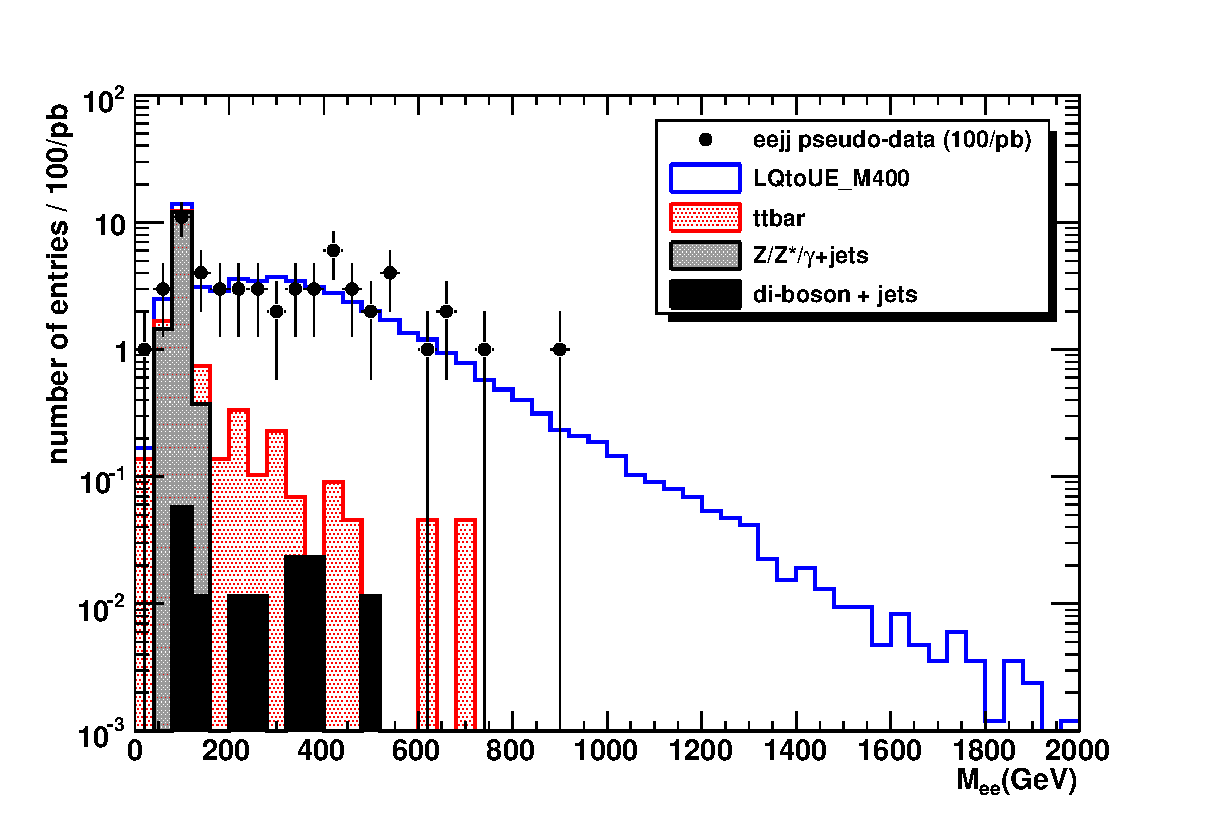
\includegraphics{plots/LQ400FullSimeejjFinalPlots/Mee_eejj_LQ400_100pb.eps}} &
      \resizebox{7.5cm}{!}{b)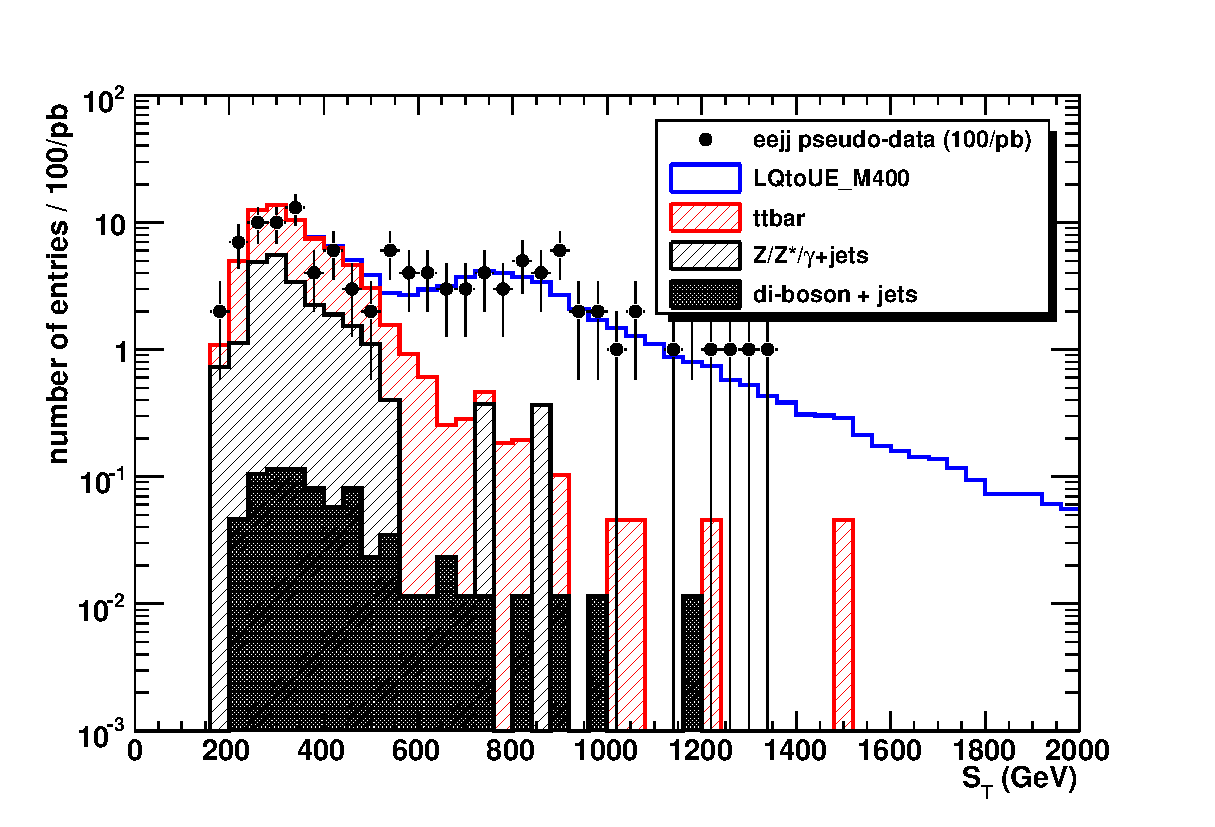
\includegraphics{plots/LQ400FullSimeejjFinalPlots/ST_eejj_LQ400_100pb.eps}} \\
    \end{tabular}
    \caption{\small \sl a) invariant mass of the electron pair, $M_{ee}$. \newline
             b) Scalar sum of the $P_T$ of the 2 leading electrons and 2 leading jets. 
	     In each histogram, the distributions for the signal with $M_{LQ}=400~$GeV 
	     and the contributing backgrounds 
	     (with the exception of the QCD background, see Section~\ref{sec:QCDBackground}) are shown after 
	     applying all cuts except the one involving the plotted variable. 
	     All histograms are summed on top of each other.
	     }
    \label{fig:Mee_St_distributions}
  \end{center}
\end{figure}


\begin{figure}[htbp]
  \begin{center}
    \begin{tabular}{cc}
      \resizebox{7.5cm}{!}{a) 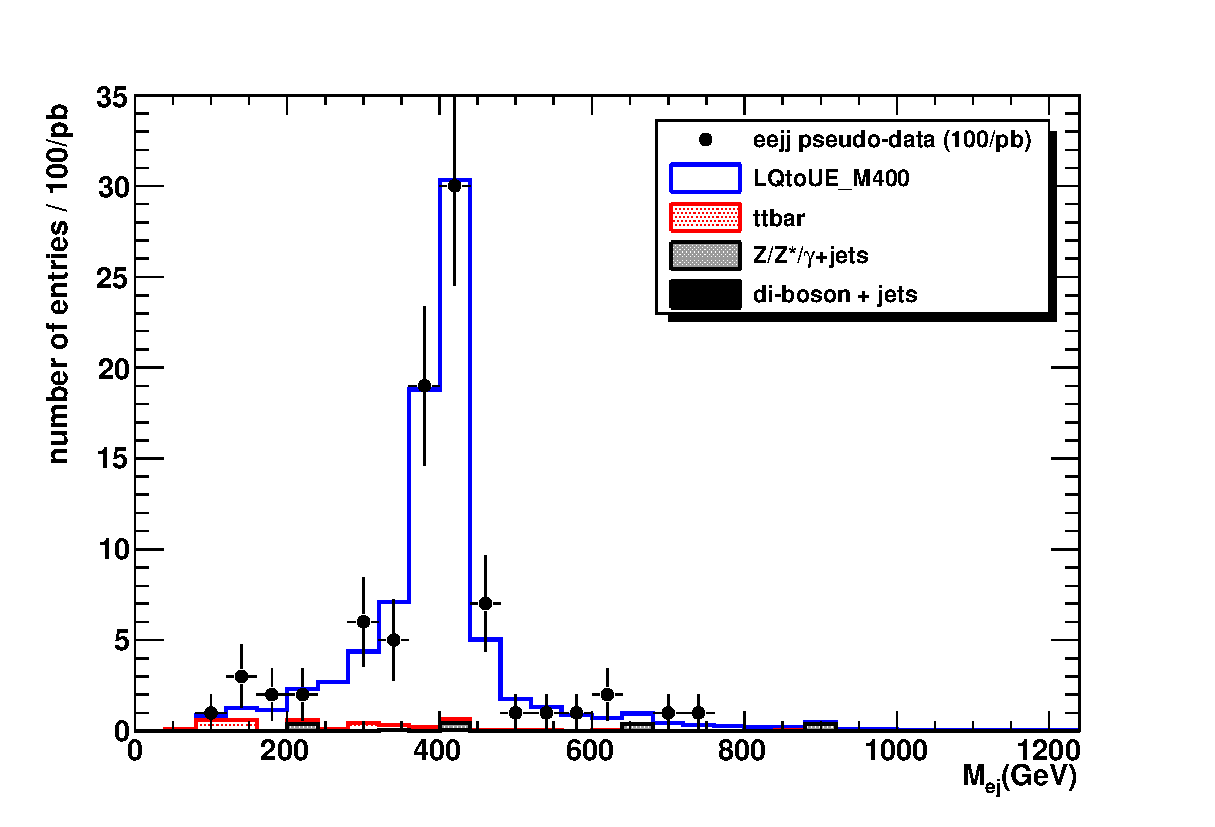
\includegraphics{plots/LQ400FullSimeejjFinalPlots/Mej_eejj_LQ400_100pb_LinScale.eps}} & 
      \resizebox{7.5cm}{!}{b) 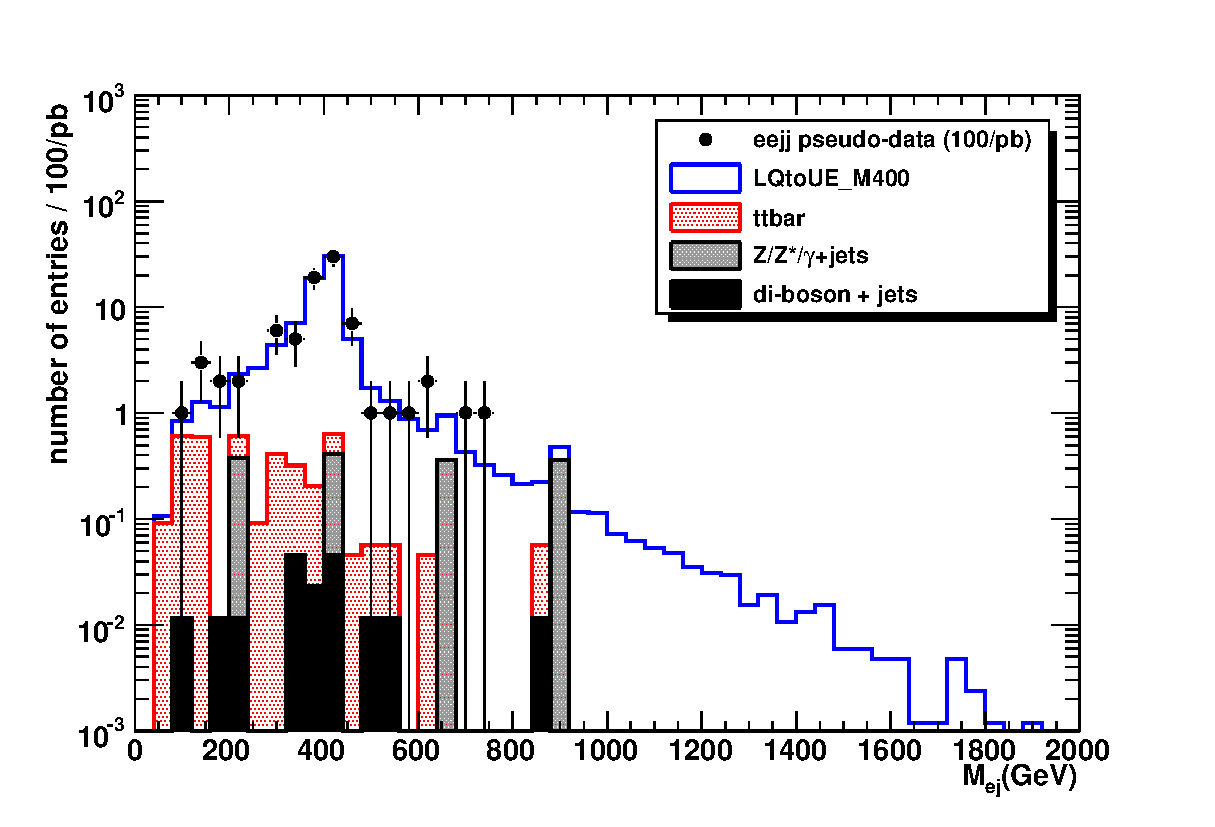
\includegraphics{plots/LQ400FullSimeejjFinalPlots/Mej_eejj_LQ400_100pb.eps}} \\
    \end{tabular}
    \caption{\small \sl Distribution of the invariant mass, $M_{ej}$, 
      of the electron-jet pairs with smaller $\Delta M_{ej}$ for the signal with $M_{LQ}=400~$GeV and the contributing backgrounds 
      (with the exception of the QCD background, see Section~\ref{sec:QCDBackground}). 
      The complete event selection has been applied.
      All histograms are summed on top of each other. 
      The plot is shown in linear and log scale in a) and b) respectively. 
      }
    \label{fig:Mej_allComb}
  \end{center}
\end{figure}


The efficiency of each selection cut is shown in Table \ref{tab:effic-MLQ400} 
for a LQ sample with a mass of 400 GeV. 


\begin{table}[htbp] 
\begin{center} 
\begin{tabular}{|c|c|c|c|} 
\hline\hline 
 Cut & $N_{evt}$ passed for $100pb^{-1}$ & $\varepsilon_{rel}$ & $\varepsilon_{abs}$ \\ 
\hline\hline 
None       &        7.50e+01       $~\pm~$       0.00e+00        &        1.0e+00       $~\pm~$       0.0e+00        &        1.0e+00       $~\pm~$       0.0e+00       \\       
       Skim       &        6.80e+01       $~\pm~$       9.00e-02        &        9.1e-01       $~\pm~$       1.3e-03        &        9.1e-01       $~\pm~$       1.2e-03       \\       
       2 ele $P_T>30~$GeV       &        6.68e+01       $~\pm~$       9.00e-02        &        9.8e-01       $~\pm~$       1.9e-03        &        8.9e-01       $~\pm~$       1.2e-03       \\       
       2 ele (ID+Iso) $P_T>30~$GeV       &        5.01e+01       $~\pm~$       1.40e-01        &        7.5e-01       $~\pm~$       3.1e-03        &        6.7e-01       $~\pm~$       1.9e-03       \\       
       2 jets (Cleaned),$P_T>$50~GeV,$|\eta|<$3       &        4.69e+01       $~\pm~$       1.40e-01        &        9.4e-01       $~\pm~$       4.1e-03        &        6.3e-01       $~\pm~$       1.9e-03       \\       
       $M_{ee}>$100~GeV       &        4.49e+01       $~\pm~$       1.50e-01        &        9.6e-01       $~\pm~$       4.5e-03        &        6.0e-01       $~\pm~$       1.9e-03       \\       
       $S_T>$620~GeV       &        3.90e+01       $~\pm~$       1.50e-01        &        8.7e-01       $~\pm~$       5.1e-03        &        5.2e-01       $~\pm~$       2.0e-03       \\       
          \hline\hline 
\end{tabular} 
\end{center} 
\caption{Sample of $M_{LQ}=400~$GeV (FullSim): Sequence of selection cuts with number of events selected in 100$~pb^{-1}$, efficiency relative to the preceding cut and absolute efficiency. The reported uncertainties on the number of events and efficiencies are statistical, due to the number of analyzed MC events.} 
\label{tab:effic-MLQ400} 
\end{table} 



 
Table~\ref{tab:selection_effic_ttbar} shows the number of events selected by each cut 
for $t\bar{t}$ and $Z/\gamma$+jet events, which are the dominant backgrounds in the eejj sample. 
A summary of the number of selected signal and background events expected in 100 pb$^{-1}$ of data 
is reported in Table \ref{tab:EventSelSummary}. 
The overall signal selection efficiencies are around 35-65\% for the LQ masses investigated. 


\begin{table}[htbp]
\begin{center}
\begin{tabular}{|c| |c|c|}
\hline
\hline
 & $t\bar{t}$ sample  & $Z/\gamma$ sample\\
 & $N_{ev}$ $100pb^{-1}$ & $N_{ev}$ $100pb^{-1}$ \\
  
\hline
\hline
None       &        4.14e+04       $~\pm~$       0.00e+00  &        4.22e+05       $~\pm~$       0.00e+00           \\       
Skim       &        6.75e+03       $~\pm~$       1.61e+01 &        9.01e+03       $~\pm~$       5.67e+01       \\       
2 ele $P_T>30~$GeV &        1.75e+03       $~\pm~$       8.77e+00&        2.65e+03       $~\pm~$       3.10e+01     \\       
2 ele (ID+Iso) $P_T>30~$GeV &        1.55e+02       $~\pm~$       2.66e+00 &        2.02e+03       $~\pm~$       2.70e+01     \\       
2 jets (Cleaned),$P_T>$50~GeV,$|\eta|<$3 &        7.72e+01       $~\pm~$       1.88e+00 &        3.28e+02       $~\pm~$       1.09e+01        \\       
$M_{ee}>$100~GeV &        4.62e+01       $~\pm~$       1.45e+00 &        2.29e+01       $~\pm~$       2.89e+00        \\       
$S_T>$620~GeV &        1.46e+00       $~\pm~$       2.60e-01 &        7.30e-01  $~\pm~$       5.20e-01        \\       
\hline
\end{tabular}
\end{center}
\caption{\small \sl $t\bar{t}$ and $Z/\gamma$ samples: the first column lists the selection sequence, $N_{ev}$ $100pb^{-1}$ is the number of selected events in $100pb^{-1}$.}
\label{tab:selection_effic_ttbar}
\end{table}


\begin{table}[htbp]
\begin{center}
\begin{tabular}{|lcc||cccc|}
\hline\hline
Signal Samples       & $S_T$ cut       & Number of Events     & Number              & of Events           & in Background    & Samples     \\
                     & (GeV)           & in Signal Samples    & $t\bar{t}$ + N jets & $Z/\gamma$ + N jets & QCD              & VV + N jets \\ 
\hline
$M_{LQ}=250~$GeV     & 460             & 342.06 $\pm$ 2.10    & 7.18  $\pm$ 0.57    & 2.55  $\pm$ 0.96    & 0.37 $\pm$ 0.37  & 0.21 $\pm$ 0.05 \\ 
$M_{LQ}=250~$GeV (*) & 460             & 359.39 $\pm$ 1.36    & as above            & as above            & as above         & as above        \\
$M_{LQ}=300~$GeV (*) & 520             & 163.37 $\pm$ 0.53    & 3.89  $\pm$ 0.42    & 1.09  $\pm$ 0.63    & 0.37 $\pm$ 0.37  & 0.15 $\pm$ 0.04 \\ 
$M_{LQ}=400~$GeV     & 620             &  38.98 $\pm$ 0.15    & 1.46  $\pm$ 0.26    & 0.73  $\pm$ 0.52    & 0.37 $\pm$ 0.37  & 0.09 $\pm$ 0.03 \\ 
$M_{LQ}=400~$GeV (*) & 620             &  40.41 $\pm$ 0.10    & as above            & as above            & as above         & as above        \\
$M_{LQ}=500~$GeV (*) & 740             &  11.56 $\pm$ 0.03    & 0.69  $\pm$ 0.18    & 0.36  $\pm$ 0.36    & 0.00 $\pm$ 0.00  & 0.05 $\pm$ 0.02 \\ 
$M_{LQ}=600~$GeV (*) & 740             &   4.04 $\pm$ 0.01    & as above            & as above            & as above         & as above        \\
%$M_{LQ}=650~$GeV (*) & 740             &   2.43 $\pm$ 0.01    & as above            & as above            & as above         & as above        \\
%$M_{LQ}=700~$GeV (*) & 740             &   1.49 $\pm$ 0.00    & as above            & as above            & as above         & as above        \\
%$M_{LQ}=800~$GeV (*) & 740             &   0.59 $\pm$ 0.00    & as above            & as above            & as above         & as above        \\
%$M_{LQ}=900~$GeV (*) & 740             &   0.25 $\pm$ 0.00    & as above            & as above            & as above         & as above        \\
%$M_{LQ}=1000~$GeV (*)& 740             &   0.11 $\pm$ 0.00    & as above            & as above            & as above         & as above        \\
\hline\hline
\end{tabular}
\end{center}
\caption{\small \sl Number events expected from LQ signal and background samples after the analysis selection for 100 pb$^{-1}$ of data.
The cut value on the kinematic variable $S_T$ depends on the LQ mass, and it is indicated in the second column.
Data samples from FullSim Monte Carlo are used for all backgrounds and for LQ masses of 250 and 400 GeV. 
Signal samples marked by (*) are made with the FastSim Monte Carlo.
The LQ cross section rapidly falls at high LQ mass, thus producing a relative decrease in the number of selected events. } 
\label{tab:EventSelSummary}
\end{table}

\subsection{Cut Optimization} \label{sec:cutOptimization}

Eight reconstructed variables are studied to optimize the selection of the events.
These are the $p_T$ of each of the two leading electrons and two leading jets, $\eta$
of the electrons, $\eta$ of the jets, the invariant mass $M_{ee}$ of the two leading electrons 
and the $S_T$ variable, the sum of the $p_T$ of the two leading electrons and jets.
The result of the optimization, performed under different LQ mass hypothesis, 
indicates $|\eta^{ele}|<2.5$, which coincides with the tracker acceptance,
and $|\eta^{jets}|<3$. The cut on invariant mass of the two electrons is found to be $M_{ee}>100$ GeV. The 
optimal cut values for electron and jet $p_T$ are consistently the lower value in the scanned range 
(20 GeV). However, the $p_{T}$ cut on electrons is moved to 30 GeV to match the one of the HEEP 
selection~\cite{HEEPNOTE}; %FIXME%
the $p_{T}$ cut on jets is moved to 50 GeV in order to reduce the effect 
of uncertainties in the initial and final state radiation, and the uncertainties 
on calorimeter response at the start-up. It is verified that such changes have a negligible effect on the signal significance. 
This optimization indicates also an $S_T$ cut 
that increases with LQ mass. 
The optimized values of $S_{T}$ cuts for different mass hypotheses are shown in Table~\ref{tab:EventSelSummary}. 


\section{Data-driven techniques for background estimate} \label{sec:bkgStudy}
After the event selection the dominant number of SM background events in the two electron 
and two jet sample (eejj sample) come from $t\bar{t}$ and $Z/\gamma$+jet processes, 
as summarized in table \ref{tab:EventSelSummary}. 
Sections~\ref{sec:ttbarControlSample} and~\ref{sec:ZcontrolSample} 
describe data-driven techniques used to estimate the absolute 
normalization for these two backgrounds, and the shape of selection variable 
distributions for $t\bar{t}$ background using control samples. 

\subsection{$t\bar{t}$ background control sample} \label{sec:ttbarControlSample}
A good control sample can be obtained by using the same selection criteria applied for the eejj sample, but 
requiring at least one electron and one muon (e$\mu$jj sample) instead of at least 2 electrons 
in the final state in addition to the two jets. 
For $t\bar{t}$ events, the selection variable distributions of the e$\mu$jj and the eejj samples
are expected to be very similar in shape since the kinematics of the process does not depend 
on the nature of the lepton. Figure~\ref{fig:ttbar} shows a good agreement between 
the shape of $M_{lj}$ and $S_{T}$ distributions with the current MC statistics available. Similar agreement 
is found also for the other reconstructed kinematic variables used in the selection. 

\begin{figure}[htb]
  \begin{center}
  \begin{tabular}{cc}
  \resizebox{8cm}{!}{a) 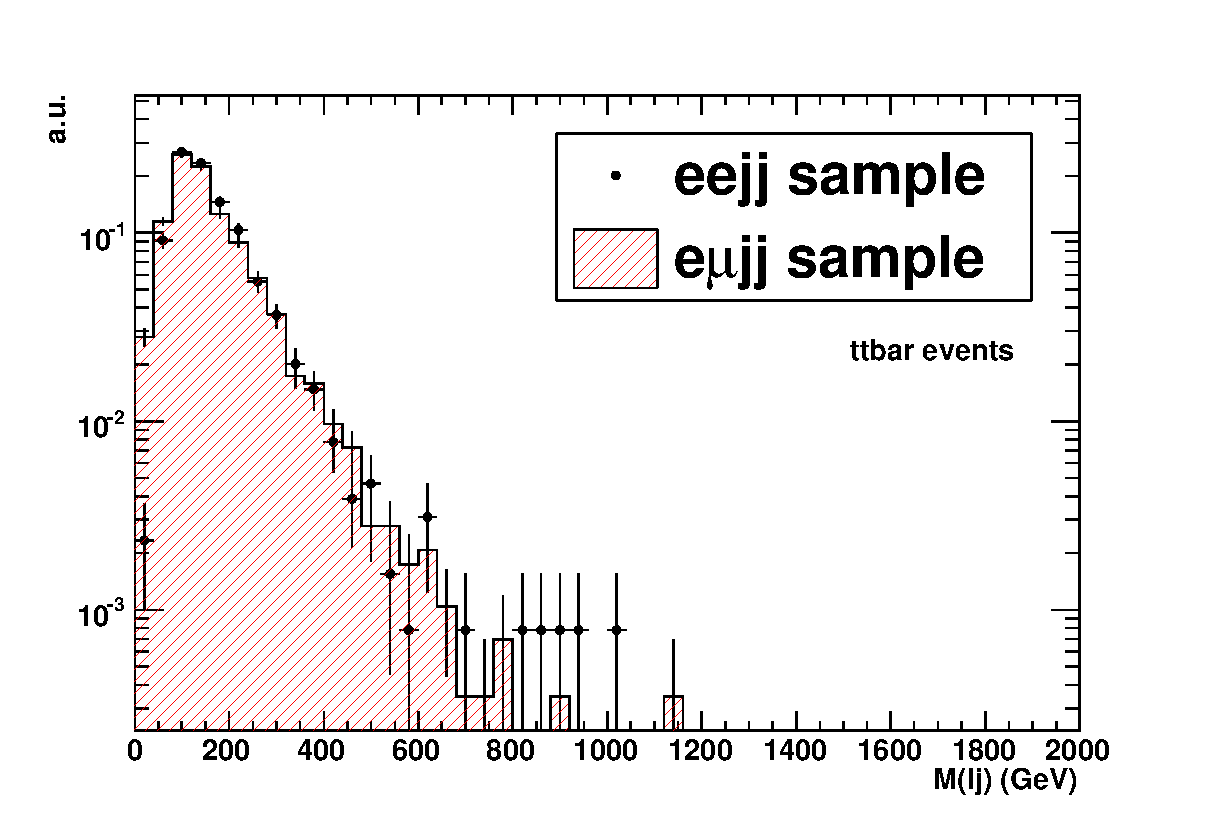
\includegraphics{plots/ttbarStudies/Mlj_eejj_VS_emujj_ttbar_STcut300.eps}} &
  \resizebox{8cm}{!}{b) 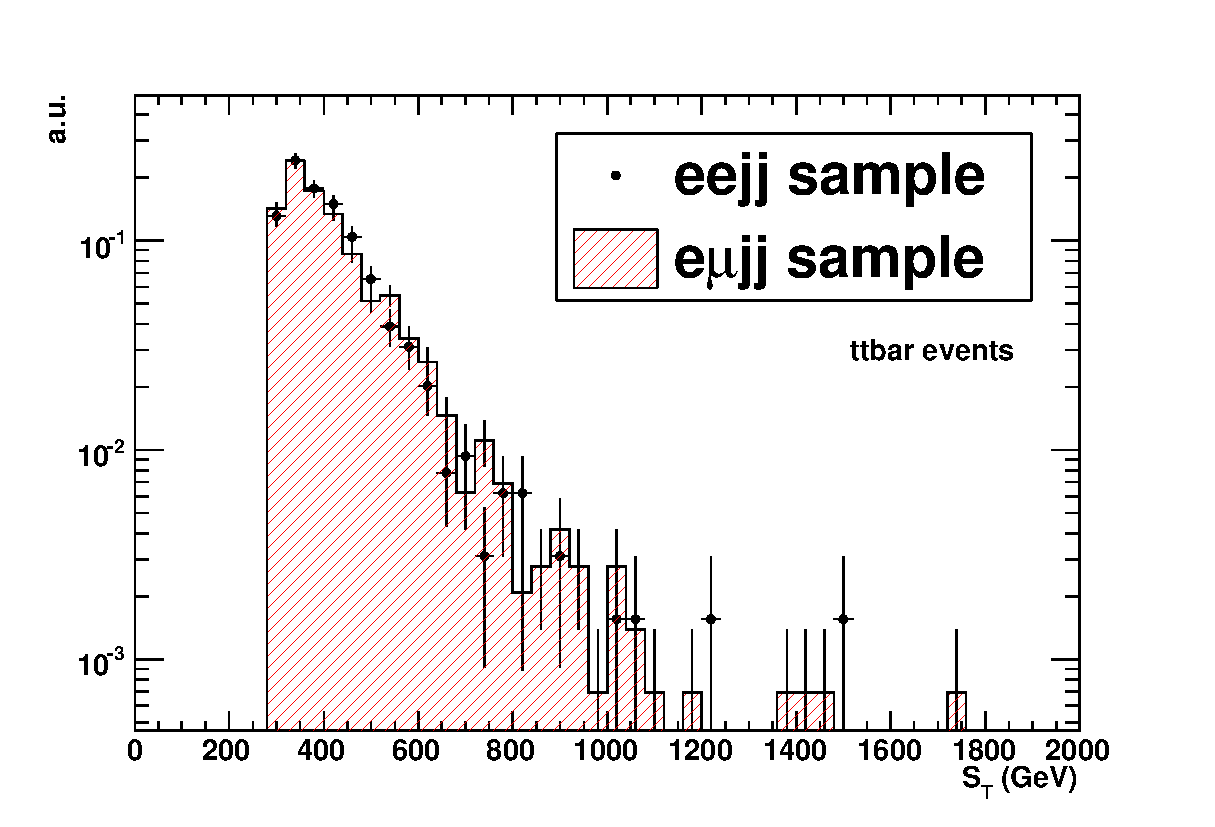
\includegraphics{plots/ttbarStudies/ST_eejj_VS_emujj_ttbar_STcut300.eps}} \\
  \end{tabular}
  \caption{\small \sl Distributions of the lepton-jet invariant mass (a) and $S_{T}$ (b) for the eejj and the e$\mu$ samples, for $t\bar{t}$ events.
  Baseline selection criteria (cut 1,2,3) 
  described in Section~\ref{sec:eventSelection} are applied, but the $S_{T}$ cut has been set to 300 GeV.}
  \label{fig:ttbar}
  \end{center}
\end{figure}

The e$\mu$jj sample is dominated by $t\bar{t}$ events, 
with a small contamination estimated from MC of less than 5\% (with $S_{T}$ cut of 300 GeV), 
mainly from di-boson events (for $W$+jets and $Z/\gamma$+jets contributions, the statistical 
uncertainties are large, around 100\%, due to limited MC statistics). 
For $t\bar{t}$ events, the e$\mu$jj sample with 100 pb$^{-1}$ of data 
is expected to have about 66, 11, and 5 events, respectively for an $S_{T}$ cut of 300, 520, and 620 GeV.

For a sample of $t\bar{t}$ events at generator level, the number of e$\mu$jj events is expected to be
exactly two times the number of eejj events, considering all the possible combinations of the $W$ decays.
In general, the trigger filter, the offline selection, and the different reconstruction efficiency,
acceptance and $P_{T}$ resolution between electron and muon put a bias in the relative amount of eejj 
and e$\mu$jj events. 
In this analysis the effect of the different reconstruction efficiency between electrons and muons 
(which is the dominant effect for the current selection) 
is considered, in order to estimate the number of eejj in the signal sample directly from 
the size of the e$\mu$jj control sample. The estimate of the number of $t\bar{t}$ events in the eejj sample, 
$N_{eejj}^{est.}$, is extracted from the e$\mu$jj sample accordingly with the relation 

\begin{equation} \label{formula:NeejFromNemujj}
N_{eejj}^{est.} = \frac{1}{2}\sum_{P_{T}^{\mu}} N_{e\mu jj}(P_{T}^{\mu}) \times R(P_{T}^{\mu}) \quad , 
\end{equation}

where $N_{e\mu jj}(P_{T}^{\mu})$ is the $P_{T}$ distribution for e$\mu$jj events of the muon  
with largest transverse momentum, and $R(P_{T})$ is the ratio between electron 
and muon reconstruction efficiencies as a function of lepton $P_{T}$. The ratio $R(P_{T})$ has been obtained 
using a MC FullSim sample of Z+jets events with an equivalent integrated luminosity of about 275 $pb^{-1}$.
The value of $R(P_{T})$ is found to be between 0.85-0.95 for $30 < P_{T} < 500$ GeV.
Once real data becomes available this ratio could be obtained with $tag\&probe$ method using $Z \rightarrow ee$ and 
$Z \rightarrow \mu\mu$ events.

\subsection{$Z/\gamma$+jet background control sample} \label{sec:ZcontrolSample}

A control sample for $Z/\gamma$+jet background estimation (eejjAtZ sample) 
can be obtained by using the same selection criteria applied for the eejj sample except 
the $M_{ee}$ cut, which is modified to select events with a real $Z$ boson reconstructed 
($80\mbox{ GeV} < M_{ee} < 100\mbox{ GeV}$). This control sample is an almost pure sample of  
$Z/\gamma$+jet events 
( less than 4\% contamination dominated by $t\bar{t}$ events, for $S_{T}$ cut of 300 GeV), 
since the cross section of the process is resonant at the Z mass. 
%the eejjAtZ sample is independent from the eejj signal sample by construction. 
For $Z/\gamma$+jet events, the eejjAtZ sample with 100 pb$^{-1}$ of data 
is expected to have about 129, 22, and 12 events, respectively for an $S_{T}$ cut of 300, 520, and 620 GeV.

%\begin{figure}[htb]
%  \begin{center}
%  \begin{tabular}{cc}
%  \resizebox{10cm}{!}{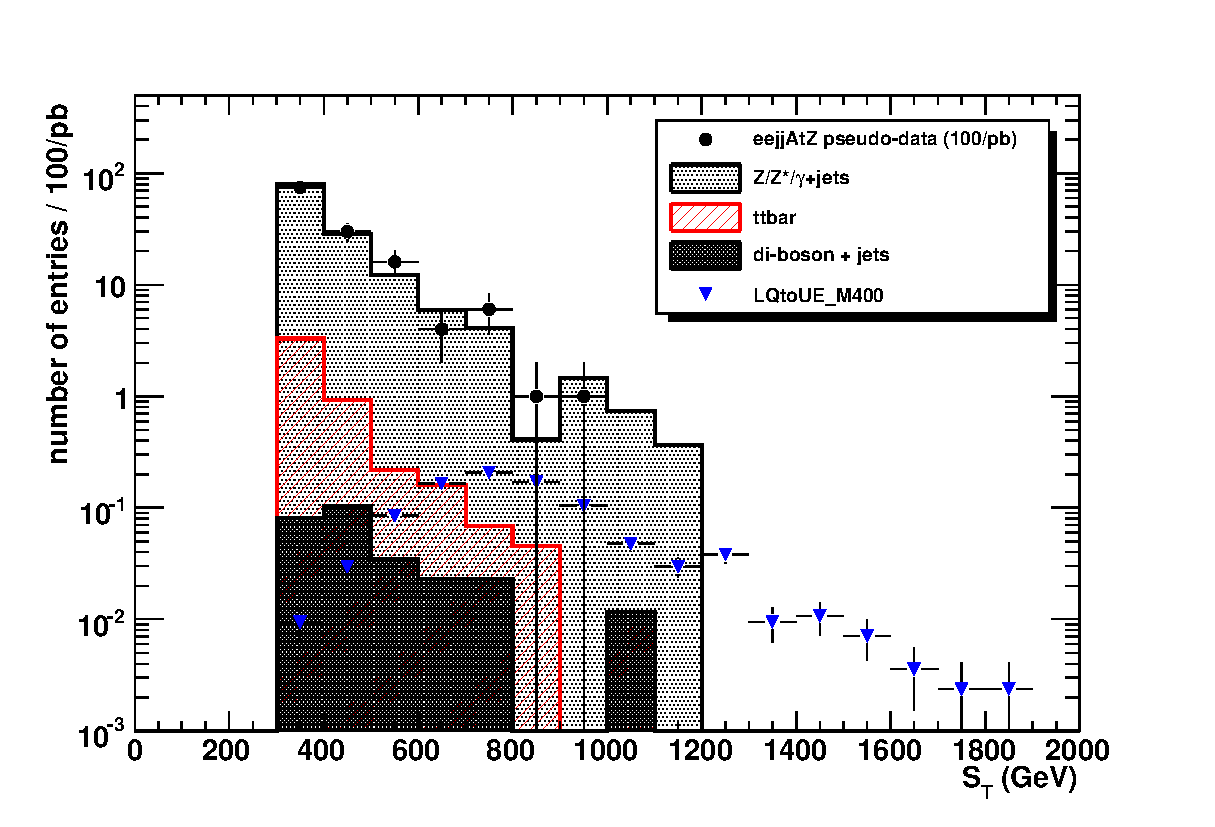
\includegraphics{plots/ZjetStudies/ST_100InVpb_eejjAtZ_looseSTcut_MeeInverted_WithLQ400.eps}} \\ 
%  \end{tabular}
%%  \caption{\small \sl Distribution of the $P_{T}$ at generator level of the electron pair ($P_{T}$ of the boson) 
%%    for $Z/\gamma$+jet events in the signal eejj sample 
%%    (cut 1,2,3,4)
%%    and the control sample (cut 1,2,4 + $80\mbox{ GeV} < M_{ee} < 100\mbox{ GeV}$), for $Z/\gamma$+jet events.}
%  \caption{\small \sl Distribution of the $S_{T}$ variable for eejjAtZ sample
%    for different background components. 
%    Histogram of signal events (at 400~GeV LQ mass) is also added. 
%    Baseline selection criteria (cut 1,2) described in Section~\ref{sec:eventSelection} 
%    are applied, $S_{T}$ cut has been set to 300 GeV, 
%    cut on $M_{ee}$ is modified to select real Z bosons ($80\mbox{ GeV} < M_{ee} < 100\mbox{ GeV}$).
%    The background histograms are summed on top of each other.
%    Black dots indicate pseudo data randomly generated accordingly with 
%    the total background distribution, and assuming 100 $pb^{-1}$ of data.}
%  \label{fig:eejjAtZContamination}
%  \end{center}
%\end{figure}
%
The rescaling of the control sample can be obtained with a hybrid method which combines the eejjAtZ data with 
MC information. Once real data is available the eejjAtZ sample can be selected. 
The number of $Z/\gamma$+jet events in the eejj signal sample ($M_{ee}>100$ GeV) can be estimated by

\begin{equation} \label{formula:NeejFromRoffZatZ}
N_{eejj}^{Z} = N_{eejjAtZ} \times R_{OffZ/AtZ} \quad , 
\end{equation}

where $N_{eejjAtZ}$ is the number of events in the eejjAtZ control sample, and 
$R_{OffZ/AtZ}$ is the ratio between the number of $Z/\gamma$+jet events 
with $M_{ee} > 100\mbox{ GeV}$ (OffZ events) and $80\mbox{ GeV} < M_{ee} < 100\mbox{ GeV}$ 
(AtZ events) that have passed all the other selection criteria.
In this analysis the value of $R_{OffZ/AtZ}$ is determined directly from MC.
%The motivations that justify this approach are discussed below:
%%
%\begin{itemize}
%%
%\item Those theoretical uncertainties that are independent 
%on the value of two electron invariant mass cancel in the ratio.
%\item For inclusive Drell-Yan production ($Z/\gamma \rightarrow ee$ with no jets), 
%the MC is expected to predict the value of this ratio with small 
%uncertainty (dominated by PDF uncertainties). 
%The data-MC comparison will be done with real data by calculating 
%the ratio $R_{OffZ/AtZ}$ using a control sample with only two electrons 
%(which is expected to be dominated by Drell-Yan events 
%up to values of $M_{ee}$ of several TeV~\cite{HEEPNOTE}).
%\item The next step will be to compare the distributions of reconstructed selection 
%variables between eejjAtZ data and MC to check the agreement in the control region.
%It is expected to have more confidence in the MC extrapolation 
%from the control region to the signal region (i.e. the estimation of the ratio $R_{OffZ/AtZ}$), 
%if the event kinematics in the two regions is not dramatically different.
%Figure~\ref{fig:STEleJetceejjAtZvsOffZ}
%show the distributions of the scalar sum of $P_{T}$ of the two leading electrons ($S_{T}^{ele}$) 
%and the two leading jets ($S_{T}^{jets}$) for $Z/\gamma$+jet events, 
%in both signal region (eejj sample) and control region (eejjAtZ control sample). 
%A significant discrepancy is observed 
%in the $S_{T}^{ele}$ distribution; this should not represent 
%a problem for the MC extrapolation, since the Electro-Weak part of the process 
%is well predicted, and the expected agreement could be directly checked with a control sample 
%of two electrons (as described in the previous bullet).
%It's also comforting that the $S_{T}^{jet}$ distributions are not dramatically different, 
%which is an indication that the hadronic part of the $Z/\gamma$+jet process 
%(the one with largest uncertainties) is similar between 
%signal and control region.  
%%
%\end{itemize}
%
%\begin{figure}[htb]
%  \begin{center}
%  \begin{tabular}{cc}
%    a.
%    \resizebox{8cm}{!}{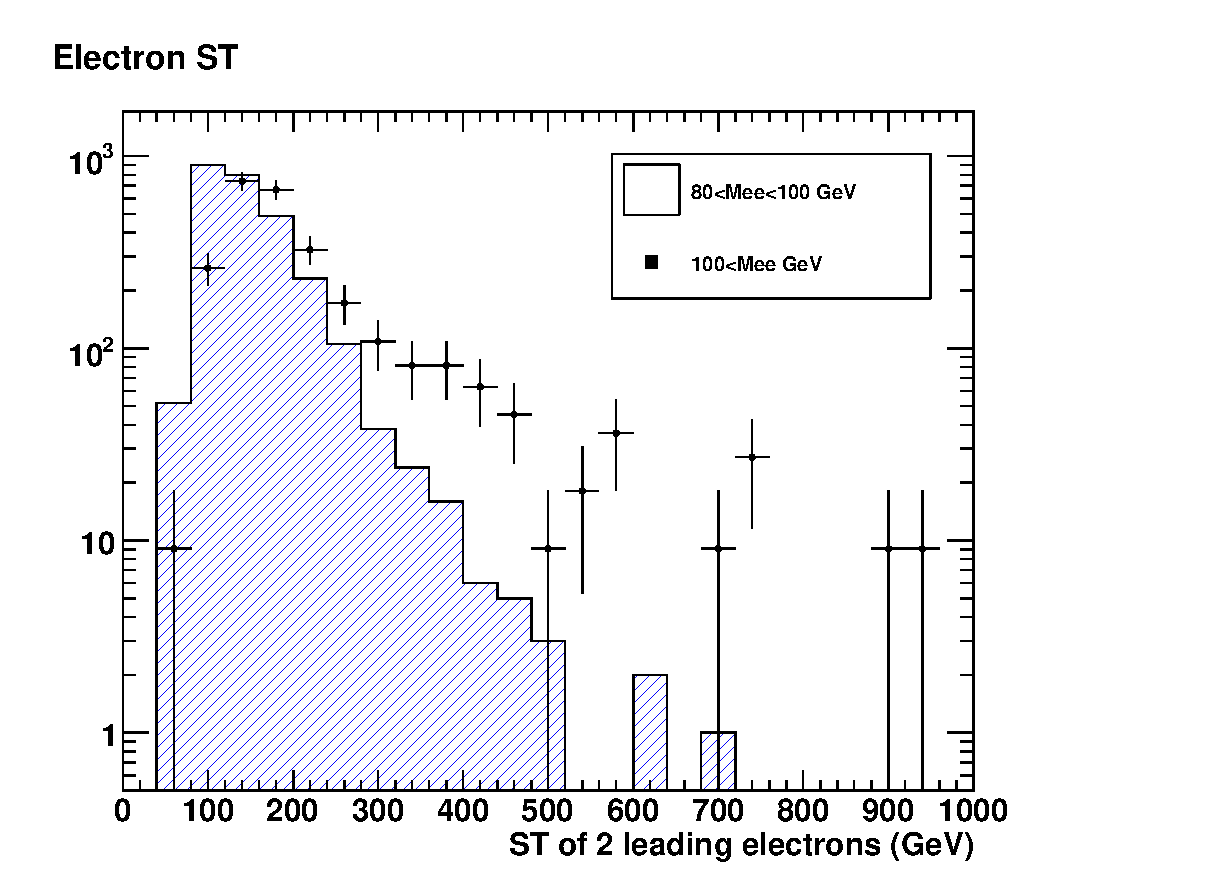
\includegraphics{plots/ZjetStudies/ST_Elecs_inside.eps}} &
%    b.
%    \resizebox{8cm}{!}{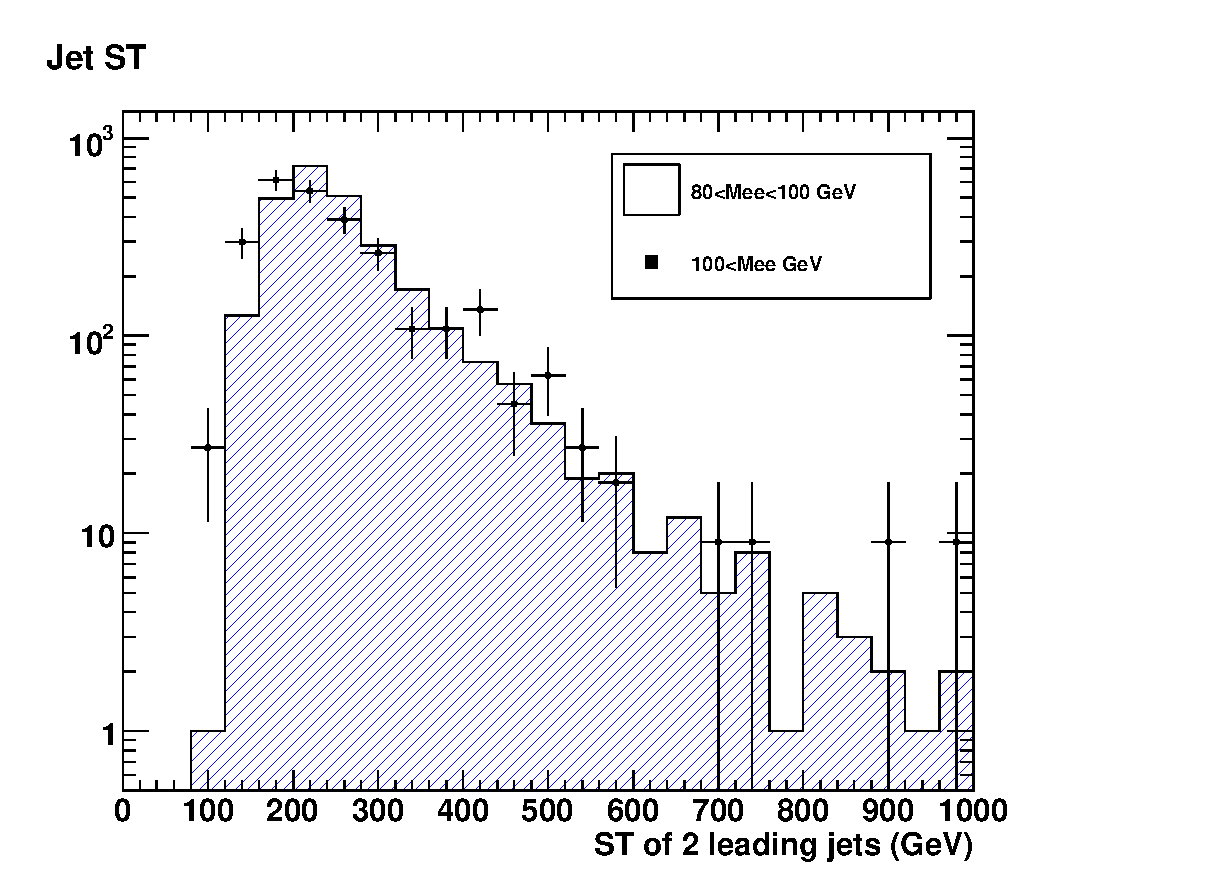
\includegraphics{plots/ZjetStudies/ST_Jets_inside.eps}} \\
%  \end{tabular}
%  \caption{\small \sl Distributions of (a) $S_{T}^{ele}$ (b) $S_{T}^{jet}$ 
%    for the signal eejj sample ($M_{ee} > 100\mbox{ GeV}$) 
%    and the eejjAtZ control sample ($80\mbox{ GeV} < M_{ee} < 100\mbox{ GeV}$), 
%    using a large FastSim sample of $Z/\gamma$+jet events.}
%  \label{fig:STEleJetceejjAtZvsOffZ}
%  \end{center}
%\end{figure}
%
%

\subsection{QCD Background} \label{sec:QCDBackground}

The MC statistics of the QCD sample is not sufficient to perform a reasonable estimate of the contamination 
of QCD events in the eejj sample, although it seems to confirm the expectation that it is small compared with 
the dominant $t\bar{t}$ and $Z/\gamma$+jet backgrounds (see Table~\ref{tab:EventSelSummary}). 
In addition, large uncertainties are expected on the cross section of QCD production at LHC start-up.
For this reason different techniques (possibly data-driven) are preferred to estimate the QCD background.

The simple approach used in this analysis is to take a QCD sample with two fake electrons and two jets (ffjj sample)
that pass all the kinematic selection criteria (see Section~\ref{sec:eventSelection}), and rescale it to estimate 
the QCD contamination in the eejj sample as
%
\begin{equation} \label{QCDRescaling}
N_{eejj}^{QCD} = N_{ffjj}^{QCD} \times {P(e|f)}^2 \quad , 
\end{equation}
%

where ``f'' is a reconstructed electron with loose ID requirements (all objects in the initial electron collection 
before applying HEEP ID and Isolation), 
``e'' is a reconstructed electron which pass all the HEEP ID and Isolation criteria (see Table~\ref{tab:HEEPselection} 
of Section~\ref{sec:electrons}), 
$N_{eejj}^{QCD}$ ($N_{ffjj}^{QCD}$) is the number of QCD events in the eejj (ffjj) sample (control sample), 
and $P(e|f)$ is the probability of a fake electron (f) to pass the HEEP ID and Isolation requirements (e).
The probability $P(e|f)$ is obtained from the rate of ``f'' to ``e'' in a ffjj sample of QCD events 
(QCD ($H_T\in[500,1000]$~GeV) is used since it's the largest contribution in the control sample) .
The number of QCD events in the eejj and ffjj sample are calculated using 
an $S_{T}$ cut of 460 GeV (which is the optimized cut for LQ mass of 250 GeV), and assuming 100 $pb^{-1}$ of data.

The probability $P(e|f)$ is found to be $\approx 2 \cdot 10^{-3}$, almost flat in the barrel region ($|\eta|<1.5$), while 
it is increasing with $\eta$ in the endcap region, up to $\approx 2 \cdot 10^{-2}$ for $|\eta|=2.5$. 
The average value $P(e|f) = 3.5 \cdot 10^{-3}$ is used.
The value of $N_{ffjj}^{QCD}$ is found to be $6130 \pm 47$. The number of QCD events in the eejj sample is estimated 
by rescaling the ffjj sample with Equation~\ref{QCDRescaling}, and it is $N_{eejj}^{QCD}=0.075$ events.
This value is in agreement with the estimate of $0.37 \pm 0.37$ events 
(see Table~\ref{tab:EventSelSummary}) obtained by directly applying the full eejj 
selection on the QCD MC sample. An uncertainty of 200\% on the value of $P(e|f)$ is estimated 
from closure tests performed with relaxed ID and Isolation cuts. 

\section{Systematic Uncertainties} \label{sec:Systematics}

The main sources of systematic uncertainties for this analysis are discussed below.
The effects of these systematic uncertainties are taken into account in Section~\ref{CMSpotential} 
by summing them in quadrature when calculating discovery and exclusion potential, unless otherwise noted.
%
\begin{enumerate}
\item Uncertainty in the jet and electron energy scale

To quantify the effect of the uncertainty on the reconstructed energy of the electron and jets
the analysis is repeated with a multiplicative factor introduced to the energy 
of jets and electrons within the event. 
A variation of the jet energy of $\pm$10\% leads to a maximum change of approximately 
7\% in the signal efficiency and 33\% in the number of background events, 
%(from $2.29 \pm 0.58$ to $3.04 \pm 0.61$ when the jet energy is {\sl increased} 10\%)
while a $\pm$5\% variation in the electron energy yields approximately a 3.5\% maximum 
change in signal efficiency and 35\% in the number of background events. 
%(from $2.29 \pm 0.58$ to $3.08 \pm 0.70$
%when the electron energy is {\sl increased} 10\%).  
%FIXME - rerun this for all mass points%
%
\item Uncertainty in the integrated luminosity of the data

This uncertainty is estimated at 10\% for the first several months of LHC running~\cite{PTDR}. 
%
\item Statistical uncertainty on the MC data

The uncertainty on the final number of selected events for the FullSim sample with a leptoquark mass of 400 GeV is 
approximately 0.4\%.  The number of events produced in the background samples, however, correspond to a much
smaller equivalent integrated luminosity than the signal samples.  
The statistical uncertainty in the number of MC events is summarized for signal and background samples 
in table~\ref{tab:EventSelSummary} of Section~\ref{sec:eventSelection}.  
%
\item Uncertainties on FastSim selection efficiencies with respect to FullSim

The signal samples produced with FastSim show a slightly higher selection efficiency than FullSim, 
mostly due to the higher reconstruction efficiency of the electrons in the FastSim. 
This leads to a higher final selection efficiency in FastSim compared to FullSim by approximately 5\% 
for leptoquark samples with a mass of 250 and 400 GeV. FullSim samples at higher mass are not available 
to perform the comparison. A conservative uncertainty of 10\% on the selection efficiency 
for FastSim samples is used in the whole mass range investigated. 
%
\item Uncertainty from the data driven background estimates

Estimates of the background by data driven techniques are affected by the statistical
uncertainties on the size of the control samples.
The number of events expected in each control sample varies with the $S_T$ cut used, as 
described in section~\ref{sec:bkgStudy}. These uncertainties can be correctly estimated 
only when data is available, and they are not included in the discovery and exclusion potential
for this analysis.
%
\item Theoretical uncertainties 

At the LHC the PDF uncertainties are expected to give the largest contribution to the theoretical uncertainties. 
The effect of this can be estimated by re-weighting 
the events based on the momentum fraction of each incoming parton.
The relative uncertainties on the differential cross sections 
typically range from 2-5\% for Standard Model processes, 
but may rise to 10\% or larger for parton processes at the TeV-scale 
(like the leptoquark pair production).
These uncertainties will be evaluated and included in future upgrades of this analysis.
\end{enumerate}



\section{CMS Discovery and Exclusion Potential} \label{CMSpotential}

In order to estimate the potential of the CMS detector to discover the first generation leptoquarks
in the electron channel, a simple counting experiment approach is used. 
The number of signal and background events expected for an integrated luminosity of
100~$pb^{-1}$ listed in Table~\ref{tab:EventSelSummary} and the systematic uncertainties described 
in Section~\ref{sec:Systematics} are used to produce the following plots. 
The QCD background estimates from Table~\ref{tab:EventSelSummary} 
are not included due to lack of MC statistics. The QCD background is expected to be 
small compared to the other main background contributions (see Section~\ref{sec:QCDBackground}).

To quantify the significance of the
leptoquark signal, $S_\text{cP}$ significance estimator~\cite{ref:scp} is used. $S_\text{cP}$ assumes a Poisson distribution
with mean $b$ and gives the probability to observe $n=s+b$ events or greater
\begin{equation}
P = p(n\geq s+b|b) = \sum_{n=s+b}^{+\infty} \frac{b^n}{n!}e^{-b},
\end{equation}
where $s$ and $b$ are the expected numbers of signal and background events, respectively. This probability is 
converted into an equivalent number of standard deviations using the one-sided Gaussian probability
\begin{equation}
P = \frac{1}{\sqrt{2\pi}}\int_{S_\text{cP}}^{+\infty} e^{-\frac{x^2}{2}}\mathrm{d}x,
\label{eq:ScP}
\end{equation}
which gives the numerical value of the $S_\text{cP}$ significance.
Figure~\ref{fig:discovery}a. shows the required integrated luminosity
for a $5\sigma$ discovery for different leptoquark mass hypotheses. 

\begin{figure}[htb]
  \begin{center}
  \begin{tabular}{cc}
  \resizebox{8cm}{!}{a. 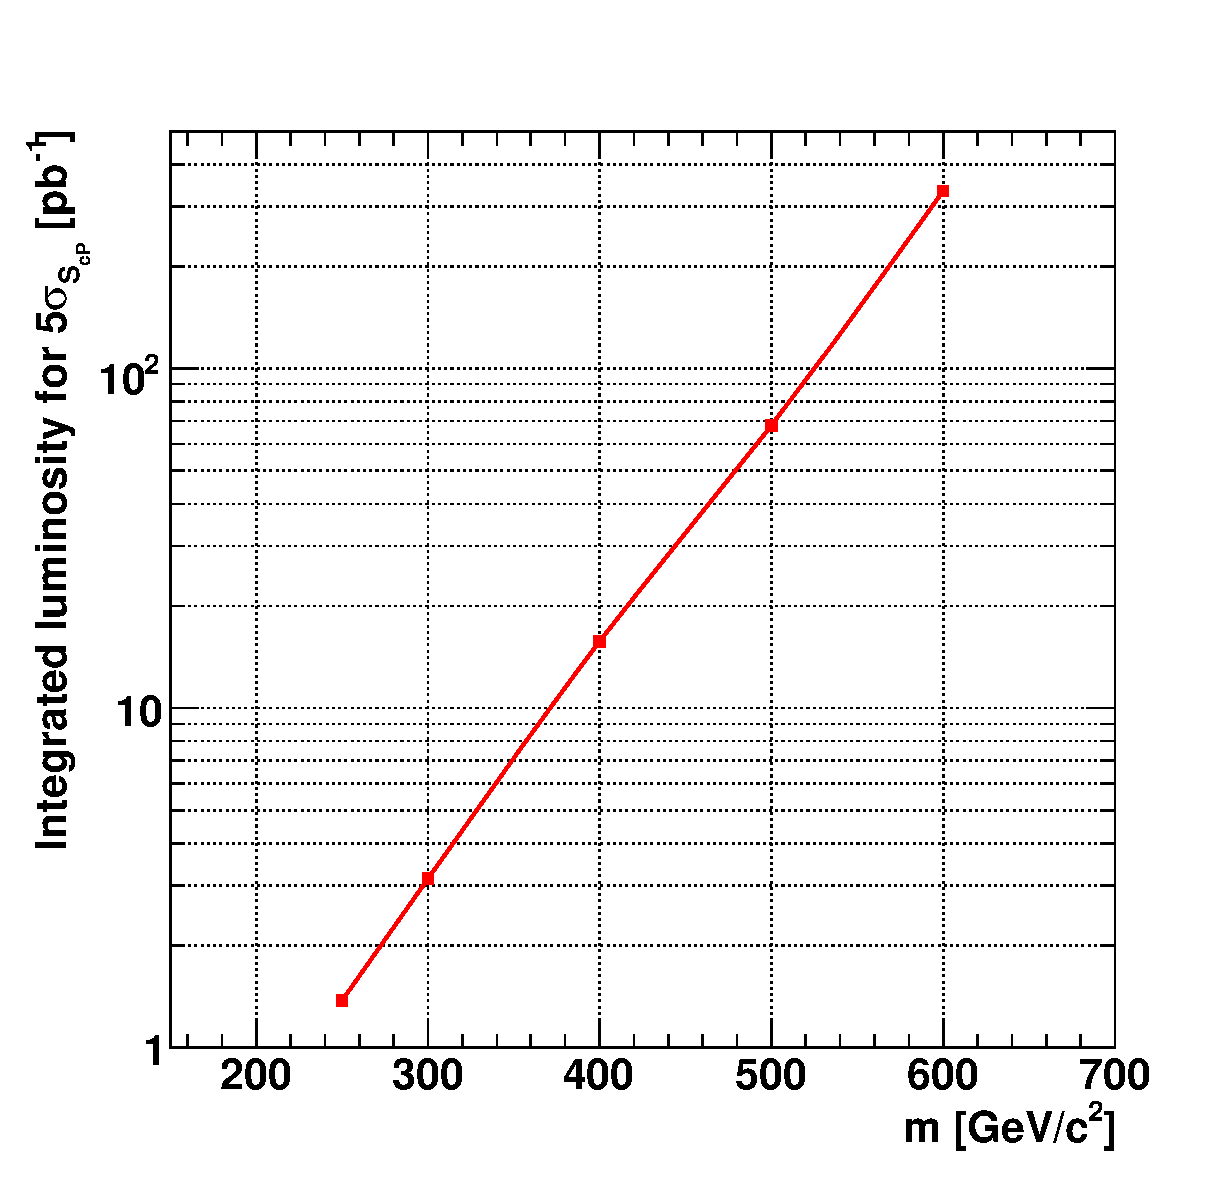
\includegraphics[width=0.5\textwidth]{plots/cmsPotential/L5sigma_vs_m_log.eps}}
  \resizebox{8cm}{!}{b. 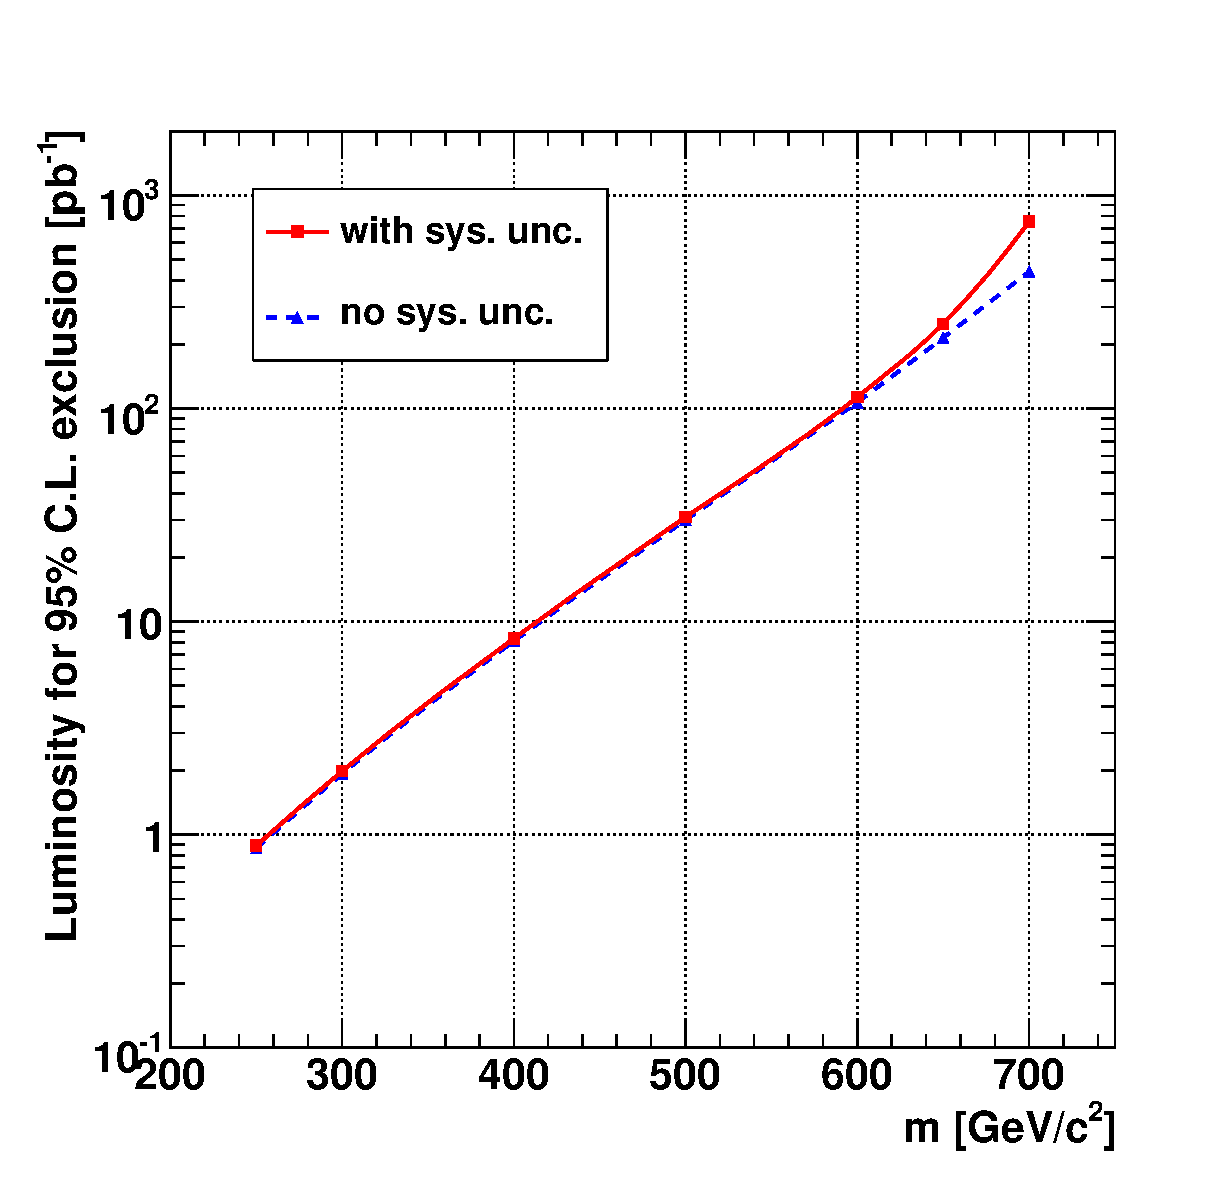
\includegraphics[width=0.5\textwidth]{plots/cmsPotential/L95CL_vs_m_log.eps}}
  \end{tabular}
 \caption{\small \sl a. Integrated luminosity
for a $5\sigma$ discovery for different leptoquark mass hypotheses assuming $\beta=1$. Solid red line includes the systematic uncertainties described in 
Section~\ref{sec:Systematics}. Shaded region is excluded by the current Tevatron limits.\newline
b. Integrated luminosity
for $95\%$ C.L. exclusion of different leptoquark mass hypotheses assuming $\beta=1$. Solid red line includes the systematic
uncertainties described in Section~\ref{sec:Systematics}. Shaded region is excluded by the current Tevatron limits.
}
 \label{fig:discovery}
  \end{center}
\end{figure}

For setting upper limits in the absence of the leptoquark signal, the Bayesian approach~\cite{ref:bayes} is used. 
Figure~\ref{fig:discovery} b. 
shows the required integrated luminosity for $95\%$ C.L. exclusion of different leptoquark mass hypotheses. 


\section{Conclusion}

The search for pair production of first generation leptoquarks that decay to
an electron and a jet has been studies using a MC simulation.
The analysis strategy and detector performance assume an integrated luminosity of 100 pb$^{-1}$ and $pp$ collisions 
at $\sqrt{s}=10$ TeV.
Standard CMS techniques are used for electron and jet identification. 
%Electron efficiencies will be determined from data using the Tag$\&$Pro [REF] technique. 
An optimized cut-based event selection has been applied.
The main expected background sources have been studied and two of them provide 
a significant contribution after event selection. 
Data-driven techniques to understand the characteristics of these contributions have been developed.

The discovery and exclusion potential in the channel with two electrons plus two jets has 
been determined using two statistical estimators suited for a counting experiment in Poissonian regime.
Effect of the main systematic uncertainties has been studied and taken into account in the final 
results. This study has shown that, 
for leptoquark masses just above the Tevatron exclusion limit of 290~GeV assuming $\beta=1$, 
an early discovery is possible with a few $pb^{-1}$ of data.
With an integrated luminosity of 100~$pb^{-1}$, discovery should be possible up
to leptoquark mass of about 500, 400, and 250 GeV assuming, respectively, 
$\beta=1$, $0.5$, and $0.1$. 
In absence of evidence of a signal, the existence of a scalar leptoquark 
with mass lower than 600 GeV and $\beta=1$ can be excluded with 100~$pb^{-1}$ of data.


%--------------------------------------
%\clearpage
%--------------------------------------

\begin{thebibliography}{}

\bibitem {theories} {D.Acosta and S.K.Blessing, Ann.Rev.Nucl.Part.Sci 49,389},
  1999,
  {\em From June 2005}
\bibitem{hera}{H1 collaboration, Search for leptoquark bosons in ep collisions at HERA}, hep-ex/0506044,
\bibitem{d02008}{Search for First-Generation Leptoquarks in the dielectron channel with the DO Detector in $p\bar{p}$ Collisions at $\sqrt{s}=1.96$ TeV}, Jun 2008,
  {\em DO Note 5644-CONF}
\bibitem{cdf2005}{Search for first-generation scalar leptoquarks in $p\bar{p}$ collisions at $\sqrt{s}=1.96$ TeV}, Sept 2005,
  {\em Phys. Rev. D 72, 051107 (2005)} (CDF paper)
\bibitem{LQSingleAndPairProd}{Leptoquark Single and Pair production at LHC with CalcHEP/CompHEP in the complete model}, Feb 2005,
  {\em arXiv:hep-ph/0502067, JHEP0509:005,2005, MSU-HEP-070204}
  
  %  \bibitem{d02007}{Searches for LQ production at D0}, Oct 2007,
  %    {\em arXiv0710.0255v1}
  
  %\cite{Mangano:2002ea}
\bibitem{MADGRAPH}
  J. Alwall et Al.
  ``MadGraph/MadEvent v4: The New Web Generation''
  [arXiv:0706.2334].
  
  %  \bibitem{Mangano:2002ea}
  %    M.~L.~Mangano, M.~Moretti, F.~Piccinini, R.~Pittau and A.~D.~Polosa,
  %    ``ALPGEN, a generator for hard multiparton processes in hadronic collisions,''
  %    JHEP {\bf 0307} (2003) 001
  %    [arXiv:hep-ph/0206293].
  %    %%CITATION = JHEPA,0307,001;%%
  
\bibitem{HeepHlt}{D. Acosta et al., The CMS High Level Trigger}, CMS AN 2007/009,
\bibitem{Kramer}{M.Kramer et al., Pair production of scalar leptoquarks at the LHC},Jan 2008 ,{\em arXiv 0411038v2}
  %\cite{Abazov:2001mx} 	 
\bibitem{GSFele}{S. Baffioni et al., Electron Reconstruction in CMS}, CMS NOTE 2006/040,
\bibitem{HEEPNOTE} {CMS Collaboration, ``Search for high mass resonance production decaying into an electron pair in the CMS experiment''}, CMS PAS EXO-08-001
\bibitem{EleID}{D. Newbold et al., Electron ID at High Energies}, CMS AN 2008/045,
\bibitem{TagAndProbe}{CMS collaboration, Measuring Electron Efficiencies at CMS with Early Data}, CMS PAS EGM-07-001 (2007),
\bibitem{JetAlg} {P. Schieferdecker et al., Performance of Jet Algorithms in CMS}, CMS AN-2008/01,
\bibitem{Abazov:2001mx} 	 
  V.~M.~Abazov {\it et al.}  [D0 Collaboration], 	 
  %``Search for first-generation scalar and vector leptoquarks,'' 	 
  Phys.\ Rev.\  D {\bf 64} (2001) 092004 	 
  [arXiv:hep-ex/0105072]. 	 
  %%CITATION = PHRVA,D64,092004;%%
  %  \bibitem{highmassToMuons}{\bf I. Altsybeev et al., Search for new high-mass resonances decaying to muon pairs in the CMS experiment}, CMS AN 2007/038,
\bibitem{JES} {R. Harris, K. Kousouris, MC Truth L2 \& L3 Factorized Jet Corrections at CMS}, CMS AN-2008/03,
\bibitem{PTDR} {CMS Collaboration 2007, CMS Technical Design Report, Volum II: Physics Performance} 
J. Phys. G.: Nucl. Part. Phys. 34 995-1579, ``Luminosity Uncertainty'' at page 1500
\bibitem{PDFRescaling} {Parton Distribution Uncertainty Determination within CMSSW - CMS AN-2009/048}, FIXME
\bibitem{ref:scp} S. Bityukov, N. Krasnikov, S. Erofeeva, and A. Nikitenko, Program for evaluation of significance,
  confidence intervals and limits by direct calculation of probabilities, PhyStat 2005, Oxford, UK 
  [http://cmsdoc.cern.ch/~bityukov]
\bibitem{ref:bayes}  C. Amsler et al., Physics Letters B667, 1 (2008), section 32.3.1
  
\end{thebibliography}

\end{linenumbers}
\end{document}
